\section{Protocol}

We will start by giving an overview of the protocol.
We have a number of participants.
We have a cothority who provide the storage in a decentralized manner.
The cothority should consist of independent actors, preferably with conflicting 
interests so that they will not collude.
We have Alice the organizer and Bob the participant who are both protesters.
We have the trustworthy journalist Jane who is present but not participating in 
the protest.
The protesters will witness each others participation proofs, e.g.\ Alice will 
witness Bob's proof and Bob will witness Alice's proof.
The result of witnessing a proof is a proof share (essentially a witness 
signature).
Jane will also participate in witnessing the protesters' proofs.
The witnessing is done through local interaction.
As soon as Alice and Bob have departed from the protest they upload their proofs 
(i.e.\ all proof shares) to the cothority for indefinite storage.
Since each proof consists of one proof share for each witness, each witness 
could potentially upload the proof share themselves to the cothority.
This would have the same effect but with added redundancy, in case Alice or Bob 
cannot upload them themselves.

We will now describe the protocol in more details.
We will describe it in the same order as outlined above:
starting with the construction of the participation proof (shares) and 
submitting the proof shares to storage.
Then we will conclude with how to verify the proofs and produce the 
participation count.

\subsection{Constructing the participation-proof shares}

An overview of the final structure of a proof is given in \cref{fig:ProofFig} 
and an overview of the communication is given in \cref{fig:ProtocolOverview}.

\begin{frame}
\begin{figure}
  \centering
  \begin{tikzpicture}[%
    -Latex,
    item/.style={rectangle,draw},
    edge from parent/.style={}
    ]
    \tikzset{%
      %grow'=left,%
      %level distance=5em%
    }
    \node[item] (proof) {Proof share}
      child {%
        node[item] (pid) {$pid$}
        child {%
          node[item] (cid) {$cid$}
          child {%
            node[item] (manifesto) {Manifesto}
          }
        }
      }
      child {%
        node[item] (wid) {$wid$}
      }
      child {%
        node[item] (ts) {$t_s$}
      }
      child {%
        node[item] (l) {$l$}
      }
      child {%
        node[item] (wsig) {$wsig$}
      }
      ;

      \path[every node/.style={font=\small}]
      (pid) edge node [anchor=south east] {$\in$} (proof)
      (wid) edge node [anchor=east] {$\in$} (proof)
      (ts) edge node [anchor=east] {$\in$} (proof)
      (l) edge node [anchor=west] {$\in$} (proof)
      (wsig) edge node [anchor=south west] {$\in$} (proof)
      ;

      \path[every node/.style={font=\small}]
      (manifesto) edge node [anchor=east] {$H(\cdot)$} (cid)
      (cid) edge node [anchor=east] {$PRF_{k_p}(\cdot)$} (pid)
      (pid) edge[bend right] node [anchor=north west] {$PRF_{k_w}(\cdot)$} (wid)
      % wsig
      (l) edge[bend right] (wsig)
      (ts) edge[bend right] (wsig)
      (wid) edge[bend right] node [anchor=north west] {$PRF_{k_w}(\cdot, \cdot, 
        \cdot)$} (wsig)
      ;

  \end{tikzpicture}
  \mode<article>{%
  \caption{%
    Structure of a proof share.
    The protester \(P\)'s identifier \(pid\) is computed using the protester's 
    key \(k_P\).
    The witness \(W\)'s identifier \(wid\) is computed using the witness's key 
    \(k_W\).
    \(t_s\) is a time interval and \(l\) is the coordinates of an area.
    The protest (cause) identifier \(cid\) is the hash value of the manifesto.
  }}%
  \label{fig:ProofFig}
\end{figure}%
\end{frame}

\begin{frame}
\begin{figure}
  \centering
  \begin{minipage}{\linewidth}
    \begin{align*}
      O\to \text{all}\colon & \text{manifesto} \\
      P\colon & pid\gets PRF_{k_P}(cid) \\
      P\to W\colon & pid \\
      W\colon & wid\gets PRF_{k_W}(pid), \\
        & wsig\gets PRF_{k_W}(wid, t_s, l) \\
      W\to P\colon & (wid, t_s, l, wsig) \\
      W\to S\colon & (pid, wid, t_s, l, wsig) \\
      P\to S\colon & (pid, wid, t_s, l, wsig)
    \end{align*}
  \end{minipage}
  \caption{%
    An overview of message exchanges.
    The organizer \(O\) broadcasts the manifesto.
    \(P\), \(W\) and their computations are as in \cref{fig:ProofFig}.
    Finally, both \(P\) and \(W\) submits the proof share to the storage \(S\).
  }%
  \label{fig:ProtocolOverview}
\end{figure}
\end{frame}

\subsubsection{Linkability and designated protest}

\Cref{CountOnce} is required to prevent Sybil attacks, i.e.\ that one individual 
can provide two participation proofs and thus be counted twice.
That situation should be detectable.
We can do this by ensuring that Alice cannot produce two valid proofs which
are unlinkable.
\Cref{DesignatedEvent} is to prevent Alice from reusing the same proof (or proof 
share) for another event.
E.g.\ there might be a counter protest at the same time and place, these would 
have the same spatial and temporal properties.
To distinguish them, we also need to prove for which of these events that a 
proof is designated.
The idea is to construct a unique identifier for a protest.

We will start with the latter.
The identifier of the protest must be regulated, for the same reasons as for the 
user identifiers --- otherwise a counter-protest can simply choose the same 
protest identifier.
As was pointed out in \cref{CauseIsTheCommonDenominator}, the cause is at the 
root of what defines a protest.
The cause can be captured in some sort of \enquote{manifesto}, thus, we will use 
the hash value of the manifesto as identifier of the protest (cause).
(As shown as manifesto and cause identifier \(cid\) in \cref{fig:ProofFig}.)

To practically propagate this identifier to the protesters the organizer can 
have a placard with a large QR code that either contains the entire manifesto or 
at least links to a website hosting the manifesto.
The user can scan this QR code with a protesting app which will automatically 
fetch it, show it to the protester for approval and then compute the identifier 
\(cid\).

Next we need to consider the protesters' identifiers to prevent Sybil attacks.
\Textcite{HowToWinTheCloneWars} created an \emph{interactive} credential system 
which allows anonymous authentication at most \(n\) times\footnote{%
  Possibly there is another scheme that makes it non-interactive, e.g.\ by 
  \Textcite{Psignatures}, see issue \#27.
}.
Alice has a \ac{PRF} key \(k\) and a blind signature on \(k\) included in her 
national identity-card (by assumption).
She will use \(k\) to compute \(pid\gets PRF_k(id)\), which is her anonymous 
identity during the protest.

\subsubsection{Temporal eligibility, created after start}

Given the properties of the storage (in \cref{StorageProperties}), for 
\cref{CreatedAfterStart}, Alice and Bob must include the hash value of an 
existing block in the blockchain in each proof share (shown as \(t_s\) in 
\cref{fig:ProofFig}).
Then it is clear that the proof must have been created after that block (since 
predicting such a value is hard).

\subsubsection{Location proofs and spatial eligibility}

\Cref{SpatiallyRelated} binds the data spatially to the location, which allows 
us to \emph{verify the data spatially}.

If we include \iac{LP}, this will tie the proof to the physical location and, 
thus, solve \cref{SpatiallyRelated}.
The \ac{LP} is \enquote{witnessed} (signed) by other participants.
The \ac{LP} contains coarse coordinates of the location, which must be within 
the protest area to be valid.
This allows Bob the protester to move within the protest area to collect 
witnesses (signatures).
It also provides privacy since the location cannot be used to deanonymize Bob's 
proof --- e.g.\ to correlate the location in his proof with captured 
surveillance footage.

\mode<presentation>{%
\begin{frame}
  \begin{figure}
    \centering
    \begin{tikzpicture}
      \tikzset{grow'=right,level distance=5em}
      \Tree [.Proof
      [.{wsig} {\(x,y\)} {$t_s$} ]
      {\dots}
      [.{wsig} {\dots} ]
      ]
    \end{tikzpicture}
  \end{figure}

  \begin{idea}[Spatial eligibility]
    \begin{itemize}
      \item Include \iac{LP} which is \enquote{witnessed} (signed) by other 
        participants.
      \item We have a coarse location, just within the protest area.
      \item This allows protesters to move around to collect signatures.
      \item This provides privacy for the location, e.g.\ cannot map to 
        surveillance cameras.
    \end{itemize}
  \end{idea}
\end{frame}
}

\mode<none>{%
\begin{frame}
  \begin{idea}[Transitive trust]
    \begin{itemize}
      \item Trusted journalist Jane attends to report.
      \item She witnesses Alice's proof.

        \pause{}

      \item Alice witnesses Bob's proof.
      \item Alice's (secret key's) transportation is physically limited.
      \item Trust on Bob's proof is proportional to time from when Jane 
        witnessed Alice's proof.
    \end{itemize}
  \end{idea}
\end{frame}

\begin{frame}
  \begin{figure}
    \centering
    \begin{tikzpicture}
      \tikzset{grow'=right,level distance=5em}
      \Tree [.Proof
      [.{wsig} {\(x,y\)} {$t_s$} [.{\color{red}tsig} {$t_s'$} ] ]
      {\dots}
      [.{wsig} {\dots} ]
      ]
    \end{tikzpicture}
  \end{figure}

  \begin{remark}
    \begin{itemize}
      \item Secret key in hardware.
      \item Alice's witness signature must depend on Jane's.
      \item High-precision relation to time?
    \end{itemize}
  \end{remark}
\end{frame}
}

We will introduce a notion of transitivity for trust in these proofs.
The \emph{trusted} journalist Jane attends the protest to report on it.
She witnesses some participants' \acp{LP}, say Alice's \ac{LP} for example.
Now Alice's \ac{LP} can be trusted as correct at that point in time.
Alice's ability to travel is physically limited.
Thus a verifier can trust any \ac{LP} that Alice witnesses proportionally to 
the time that has passed since Jane witnessed Alice's \ac{LP}.
We can apply this argument recursively for any other participant's \ac{LP} that 
Alice has witnessed.
However, this requires some assumptions:
\begin{itemize}
  \item It is actually Alice's signing key must have physically limited travel.
    This can be assumed for signing keys that are embedded into hardware by 
    some trusted person.
  \item Alice's witness signature must depend on Jane's witness signature, to 
    prove that Alice signed after Jane.
\end{itemize}
\begin{remark}
  This probably requires high-precision timestamps, i.e.\ a trusted 
  time-stamping server must be available during the protest.
  Or the proofs must be submitted to the \ac{tposet} during the protest.
\end{remark}

\subsubsection{Temporal eligibility, created before end}

Given the properties of the storage system in \cref{StorageProperties}, 
\cref{CreatedBeforeEnd} is straight-forward: Alice and Bob simply commit their 
proofs to the blockchain as soon as possible after they have participated in the 
protest.
Thus we can infer that a proof (or proof share) was created at the latest when 
it was committed.

\subsection{Verifying the proofs}

Alice must also provide \iac{NIZK} proof that \(pid = PRF_k(id)\) and that she 
knows a signature by the identity authority on \(k\).
Thus \(pid\) will be used as the unique identifier in the proof shares (and all 
computations below) whereas the \ac{NIZK} proof will be used separately to prove 
the validity (eligibility) of \(pid\).

If the proofs are stored publicly, then an individual can check that their 
proof has been included (committed) there.
Thus \cref{IndividualVerif} is fulfilled.
Similarly for universal verifiability.
If the storage is public, then anyone can download all the proofs, verify their 
eligibility and count them.
Thus anyone can verify the result, which fulfils \cref{UniversalVerif}.

\mode<presentation>{%
\begin{frame}
  \begin{idea}[Individual verifiability]
    \begin{itemize}
      \item Proofs are stored (committed) publicly.
      \item Each participant can check that their proof is indeed included.
    \end{itemize}
  \end{idea}

  \pause{}

  \begin{idea}[Universal verifiability]
    \begin{itemize}
      \item Proofs are stored (committed) publicly.
      \item Anyone can download all proofs, verify eligibility and then count 
        them.
    \end{itemize}
  \end{idea}
\end{frame}
}

\subsubsection{Participation-proof privacy}

A demonstration is very different from voting in one sense: at a demonstration, 
Alice must be physically present and that very presence shows her support for 
the cause.
In voting, on the other hand, everyone is present and Alice has multiple 
options which are not revealed by her mere presence.
% XXX Check if unlinkable is the correct term
Hence, if Alice submits a proof of participation, the proof must be unlinkable 
to Alice, yet, if Alice submits another proof, those two proofs must be 
linkable (due to eligibility verification, \cref{EligibilityVerif}) so that 
Alice is not counted twice.
This is fine, since we do not want to catch any cheater, we just do not want to
count them more than once.

\mode<presentation>{%
\begin{frame}
  \begin{remark}
    \begin{itemize}
      \item Voting: different alternatives when participating.
      \item Protesting: participation implies the alternative.
    \end{itemize}
  \end{remark}

  \pause{}

  \begin{idea}[Proof privacy]
    \begin{itemize}
      \item Eve shouldn't be able to link Alice's published proof back to 
        Alice.
      \item But if Alice publishes two proofs, those two are linkable.

        \pause{}

      \item We're not interested in unmasking trolls, just not count them more 
        than once.
    \end{itemize}
  \end{idea}
\end{frame}
}

\begin{frame}
  \begin{remark}
    Unique ring signatures~\cite{UniqueRingSignatures} has this property: two 
    signatures are linked with high probability.
  \end{remark}

  \begin{question}
    Can we link a verified key to a unique ring signature key?
  \end{question}

  \pause{}

  \begin{question}
    How to submit the proofs to the system?
  \end{question}
\end{frame}

\subsubsection{Receipt freeness}

Receipt freeness implies that Alice enjoys deniability against Eve:
Eve should not be able to use the published proof to tie it to Alice, even if 
Eve has access to Alice's device (i.e.\ all her private keys).
E.g.\ Eve should not be able to reproduce the same proof and thus verify that 
Alice has created one of the proofs.

\mode<presentation>{%
\begin{frame}
  \begin{remark}
    \begin{itemize}
      \item The proof itself is a sort of receipt.
        
        \pause{}

      \item If Eve compromises Alice's device, she can use it to verify that 
        she participated.

        \pause{}

      \item We need a signature scheme that cannot reproduce the same signature 
        when run on the same inputs.
    \end{itemize}
  \end{remark}
\end{frame}
}

\begin{frame}
\mode<presentation>{%
  \begin{idea}[Receipt freeness (deniability)]
    \begin{itemize}
      \item Alice submits her proof.
      \item She stores the hash of the head of the \ac{tposet}.
      \item She removes the proof and signature key.

        \pause{}

      \item E.g.\ a short-term and a long-term credential, then Alice can 
        drop the short-term credential.

      \item But Alice should still not be able to participate twice.
    \end{itemize}
  \end{idea}
}

  \pause{}

  \begin{question}
    Is there such a signature scheme?
    Can we construct it?
  \end{question}
\end{frame}

Say that Alice submits her proof and stores the hash of the head of the 
\ac{tposet} after her proof is included.
Now she can remove her proof and just keep the hash to verify that her proof is 
still there.
She can also remove her signature key, so that Eve cannot use it to reproduce 
the signature using the same inputs.


\subsubsection{Architecture}

We also have an architectural problem.
If the system is only run by volunteering activists, then Eve can simply 
analyse network traffic and look for people running nodes in the system.

\begin{question}
  Shall we offer a platform that is run by a variety of institutions who 
  offers to verify protests?
  Or go strictly peer-to-peer?
\end{question}

\begin{question}
  If strictly peer-to-peer, and only run by protesters, one can infer that 
  they are protesters by running such a node.
  Can this be mitigated?
\end{question}

Similarly, we have the problem of how protesters submit their proofs to the 
system.
This must be done anonymously.
Otherwise Eve can analyse the network traffic to find out who submitted proofs 
to the system.
The main problem here is that the participants must be indistinguishable from 
non-participants.
This means that we cannot use special-purpose anonymizing 
technologies.

\begin{question}
  How do we submit the proofs to storage?
  Voting normally uses mix-nets (provable shuffles).
\end{question}

\begin{remark}
  We must mix participants with non-participants.
\end{remark}

